\documentclass{article}
\usepackage{amsmath}
\usepackage{amssymb}
\usepackage{color}
\usepackage{graphicx,epsfig}
\usepackage[latin1]{inputenc}
%\usepackage[francais]{babel}
\usepackage{subfigure}
 \usepackage{psfrag}

\usepackage{url}
\usepackage[squaren,Gray]{SIunits}


\setlength{\textwidth}{16cm}
\setlength{\textheight}{22cm} 
\setlength{\oddsidemargin}{0cm}

%\renewcommand{\baselinestretch}{2.0}
%\DeclareMathOperator{\argmin}{argmin}
\DeclareMathOperator{\argmax}{argmax}
\DeclareMathOperator{\minimize}{minimize}
\DeclareMathOperator{\support}{supp}
%\DeclareMathOperator{\proj}{proj}
%\DeclareMathOperator{\sgn}{sgn}
%%%%%%%%%%%%%%%%%% Ajout Vincent
%\usepackage{rotating}
\usepackage{algorithmic}
\usepackage{algorithm}
%\newcommand{\Frac}[2]{\displaystyle \frac{#1}{#2}}
%\renewcommand{\baselinestretch}{2.0}                                                                               
%\newcommand{\contract}{{\,\Bar{\Bar\otimes}\,}}
%\newcommand{\scontract}{{\,{\Bar\otimes}\,}}
%\newcommand{\tcontract}{{\,{\Bar{\Bar{\Bar\otimes}}}\,}}

\input{macro.tex}
\usepackage{showlabels}
\usepackage{fancyhdr}\usepackage{lastpage}

\fancyhead[L]{\texttt{Acary Brogliato -- Euler Sliding}}
\fancyhead[C]{}
\fancyhead[R]{\texttt{\thepage/\pageref{LastPage}}}
\fancyfoot[L]{}
\fancyfoot[C]{}
\fancyfoot[R]{\texttt{file EulerSliding.tex -- \isodayandtime}}


\begingroup
\count0=\time \divide\count0by60 % Hour
\count2=\count0 \multiply\count2by-60 \advance\count2by\time
% Min
\def\2#1{\ifnum#1<10 0\fi\the#1}
\xdef\isodayandtime{\the\year-\2\month-\2\day\space\2{\count0}:%
\2{\count2}}
\endgroup





\usepackage{pifont}
\def\cqfd{\ifmmode\sqw\else{\ifhmode\unskip\fi\nobreak\hfil
\penalty50\hskip1em\null\nobreak\hfil\ding{111}
\parfillskip=0pt\finalhyphendemerits=0\endgraf}\fi}

\makeatother


\def\geq{\geqslant}
\def\leq{\leqslant}





%%%% fin macro %%%%
%%%%%%%%%%%%%%%%%% End Ajout Vincent



\newtheorem{definition}{Definition}
\newtheorem{proposition}{Proposition}
\newtheorem{lemma}{Lemma}
\newtheorem{claim}{Claim}
\newtheorem{remark}{Remark}
\newtheorem{assumption}{Assumption}
\newtheorem{example}{Example}
\newtheorem{conjecture}{Conjecture}
\newtheorem{corollary}{Corollary}
\newtheorem{OP}{OP}
\newtheorem{problem}{Problem}
\newtheorem{theorem}{Theorem}

\newcommand{\CC}{\mbox{\rm $~\vrule height6.6pt width0.5pt depth0.25pt\!\!$C}}
%\newcommand{\ZZ}{\mbox{\rm \lower0.3pt\hbox{$\angle\!\!\!$}Z}}
%\newcommand{\RR}{\mbox{\rm $I\!\!R$}}
%\newcommand{\NN}{\mbox{\rm $I\!\!N$}}
\newcommand{\Qend}{\hfill $\Box$}

%\newcommand{\ie}{i.e.}
%\newcommand{\eg}{e.g.}
%\newcommand{\cf}{c.f.}



\def\Er{{\rm I\! R}}
\def\En{{\rm I\! N}} 
\def\Ec{{\rm I\! C}}
\def\dT{{\rm {\it d}\! \ll T \gg}} 
\def\dll{{\rm {\it d}\! \ll}} 
%\font\tete=cmr8 at 8 pt
%\font\titre= cmr12 at 20 pt 
%\font\titregras=cmbx12 at 20 pt





\begin{document}

\pagestyle{fancy}

\title{Time-stepping numerical simulation of switched circuits with the non-smooth dynamical systems approach} 

\author{Vincent Acary, Olivier Bonnefon, Bernard Brogliato \\ \\ INRIA, Bipop team-project \\ ZIRST Montbonnot \\ 655 avenue de l'Europe
\\ 38334 Saint Ismier cedex, France \\ \\  Vincent.Acary@inrialpes.fr, Olivier.Bonnefon@inrialpes.fr, Bernard.Brogliato@inrialpes.fr}




\maketitle 

\thispagestyle{fancy}


{\bf Keywords:} Switching circuits, complementarity problems, backward Euler algorithm, power converters, complementarity dynamical systems, analog simulation, multivalued systems, unilateral state constraints. IEEE EDICS: CAD160A0


\begin{abstract}

\end{abstract}



\section{Introduction}



It is well know that conventional accurate analog simulation tools, which are based on the Newton-Raphson nonlinear solver, can have serious drawbacks when they are used for the integration of non-smooth circuits, containing switches and piecewise linear components (like ideal diodes and transistors). This is especially true when the number of events becomes too large, or when sliding modes exist, which is common in practice. Then analog (SPICE-like) tools  may become very time consuming, or provide very poor results with chattering \cite{galias2006}, or even fail \cite{maffezzoni2006,yuan2003,mayaram2000,chung1994,biolek2007}. The same applies to ``hybrid'' integrators that consider an exhaustive enumeration of all the system's modes, which have a very limited scope of application because of the exponential growth of the number of modes that have to be simulated separately. Along the same lines, event-driven schemes can hardly simulate systems with large number of events, because they soon become quite time-consuming and do not allow for accumulations of events \cite{acary-brogliato2008}. 

It is therefore clear that other types of numerical schemes have to be applied for highly non-smooth switching circuits. Since a numerical method always relies on a specific modelling approach, a logical path is to first reconsider the models of non-smooth components (diodes, switches, transistors, {\em etc}) so that efficient numerical solvers can be applied. The non-smooth dynamical systems (NSDS) approach, which is the one chosen in this paper, appears to be a suitable framework for the simulation of non-smooth circuits, allowing one to efficiently simulate systems with very large number of events, and sliding mode trajectories. It consists of modelling non-smooth components as piecewise linear functions, with possible vertical branches (inducing some unilaterality in the system, hence possible state jumps, when these branches are infinite). The time-discretization of such non-smooth systems then yields various types of so-called one-step-non-smooth-problems (OSNSP), for instance complementarity problems or quadratic programs with equality-inequality constraints, which require specific solvers. The NSDS approach may then take advantage of the quite important works that have been led by the Nonlinear Programming community concerning the development of efficient solvers for complementarity problems \cite{facchinei} and optimization tools \cite{hiriart1992}, and also by the Contact Mechanics community \cite{acary-brogliato2008}, where Moreau and Jean developed the so-called Non-Smooth Contact Dynamics (NSCD) method within the theoretical framework of Moreau's sweeping process \cite{moreau1988,jean1999,moreau1999}. The numerical method that is used in this paper, owes a lot to the NSCD method of mechanics, and will be named {\em Moreau's time-stepping scheme}. As alluded to above, non-smooth components are often represented with piecewise-linear functions, or with complementarity relations, or with inclusions into normal cones. The piecewise-linear modelling approach in non-smooth electrical circuits has been pioneered by Chua et al  in \cite{chua1978,chua1983,chua1985}, and complementarity problems have been introduced in \cite{bokhoven1978,stevens1981,vandenberghe1989}, followed by the works of Leenaerts and van Bokhoven \cite{leenaerts1999,leenaerts-bokhoven1998}, Vlach et al \cite{vlach1997,vlach1995a,vlach1995b}. Camlibel et al \cite{frasca2008,camlibel2002} studied the convergence of backward Euler methods, and comparisons with other (analog and hybrid) integrators are proposed in \cite{vasca2009}. Glocker et al \cite{glocker2005,moller2007} led interesting developments showing the analogy between mechanics and electricity for various types of non-smooth components, and also proposed a time-stepping method inspired by Moreau's algorithm for contact mechanics (consequently quite close to the algorithm used in this paper). Variational inequalities of the second kind were recently introduced in electronics in \cite{adly2007,goelevenJOTA,addi2009} to study the existence and uniqueness of solutions for static circuits, or the equilibria of dynamical circuits with non-smooth devices. Other works may be found in \cite{enge2005,batlle2005,giaouris2008}.


The objective of this paper is twofold: first it is shown on an academic example taken from \cite{maffezzoni2006} that the NSDS approach allows one to simulate a non-smooth system for which conventional analog methods fail (roughly speaking, the iterative solver for complementarity problems converge, whereas Newton-Raphson does not); second, numerical results for a buck converter are presented and comparisons with other (analog and hybrid) tools are done. The buck converter example in fact demonstrates on a significant case study that the proposed time-stepping method is efficient for systems with a large number of events. Compared to previous works \cite{glocker2005,vasca2009}, the ideal switches are here modelled and simulated for the first time in a completely implicit way, the advantage of which will be explained.  The simulations are done with the {\sc siconos} software platform\footnote{http://siconos.gforge.inria.fr/} of the INRIA \cite{acary-brogliato2008,Acary-Perignon2007,mathmod}, that is an open-source software package dedicated to non-smooth dynamical systems described by complementarity relations. The paper is organized as follows: in section \ref{section2} the modelling and general time-discretization frameworks are recalled; in section \ref{section3} an elementary closed-loop switching circuit taken from \cite{maffezzoni2006} is simulated; in section \ref{section4} the buck converter example is treated and comparisons are presented. Conclusions end the paper. 



\paragraph{Notation:} normal cone, projection, LCP, MLCP, NLCP,




\section{The non-smooth dynamical equations}
\label{section2}

\subsection{Non-smooth electronic devices modelling}
\label{section21}

The NSDS approach for the  modelling of piecewise linear components in electrical circuits has been described in detail  in several of the above cited publications, and will just be recalled here for the sake of readability. Depending on one's tastes, the current-voltage law of non-smooth electronic devices may take the form of various types of complementarity relations, or of inclusions into normal cones, or more generally of inclusions like $v \in {\cal F}(i)$ for some set-valued function ${\cal F}: \RR \rightarrow \RR$ \cite{adly2007,glocker2005}. Let us provide details on three non-smooth devices that will be used in the next examples of sections \ref{section3} and \ref{section4}. 

\paragraph{Non-smooth  diodes:}  The notation for the currents and the potentials at the ports of
the diode is depicted on figure \cite{fig:DIODE}.

\begin{figure}
  \centering
  \input{./figure/diode.pstex_t}
  \caption{diode Symbol}
  \label{fig:DIODE}
\end{figure}


Four models of diodes are depicted in figure \ref{figdiodes}: the smooth exponential model in figure \ref{figdiodes} (a), ideal diodes with possible residual current $-a$ and voltage $-b$ in figure \ref{figdiodes} (b), and the ``hybrid'' model which considers the two modes separately with an associated script in figure \ref{figdiodes} (c). The piecewise-linear model in figure  \ref{figdiodes} (b) is chosen in this paper. The drawbacks of the Shockley law is that it introduces stiffness in the dynamical equations. The hybrid model becomes rapidly unusable if the number $m$ of diodes increases, since the number of modes to be described in the associated script varies as $2^{m}$. This will be shown on the converter example. On the contrary the ideal model of figure  \ref{figdiodes} (b) yields, when introduced in the dynamics, complementarity problems or equivalently inclusions into normal cones, that yield time-stepping methods for which efficient solvers exist. Showing the efficiency of these methods is the object of this paper.

\begin{figure}
 \begin{center}
    \begin{tabular}{cccc}
      smooth modeling & non-smooth modeling & hybrid modeling &equivalent resistor model\\ \\
      \scalebox{0.5}{\input{./figure/shockleylaw.pstex_t}}
      &   \scalebox{0.5}{\input{./figure/figdiode.pstex_t}}
      &  \scalebox{0.6}{\input{./figure/hybrid_diode.pstex_t}}
      &  \scalebox{0.6}{\input{./figure/diodeReq.pstex_t}}\\ 
  \mbox{{\footnotesize    $ i(t) =  i_s \exp(- \frac{v(t)}{\alpha} - 1  $}}
      & \mbox{{\footnotesize $ 0\leq i(t)+a \perp v(t)+b \geq 0  $ }}
      &
\mbox{{\footnotesize  $\begin{array}{clc}
        \mathsf{off} &=& \mathsf{s} < 0 \\
       v(t)  &=& \mathbf{if}\quad \mathsf{off} \quad \mathbf{then}\quad \mathsf{-s}\quad \mathbf{else} \quad 0 \\
       \ i(t) &=& \mathbf{if}\quad \mathsf{off} \quad \mathbf{then}\quad 0
        \quad \mathbf{else}\quad \mathsf{s}
      \end{array} $ }}
      &
\mbox{{\footnotesize  $v(t)=\left\{\begin{array}{ll} R_{off}\; i(t) & \mbox{if}\;v(t) < 0 \\   R_{on}\; i(t) & \mbox{if}\;v(t) \geq  0  \end{array}\right.$ }}
\end{tabular}
  \end{center}
\caption{four models of diodes.}
\label{figdiodes}
\end{figure}

\begin{ndrob}
  Using the model \ref{figdiodes} (b) leads a condition number of the MLCP matrix near
  $\frac{R_off}{R_on}$, that cause trouble with the Fisher-Burmeister algorithm.\\
  Using \ref{figdiodes} (b) leads to smaller condition number of the system.
\end{ndrob}

Quite similar developments and comments may be made for ideal Zener diodes, piecewise linear practical diodes and practical Zener diodes, see e.g. \cite{acary-brogliato2008,addi2009}. 


%\begin{figure}
% \begin{center}
% \leavevmode
% \input{figdiode.pstex_t}
% \caption{An ideal diode with residual voltage and current.}
% \label{figdiode}
% \end{center}
%\end{figure}


\paragraph{Non-smooth switches:}The notation for the currents and the potentials at the ports of
the ideal switch is depicted on figure \cite{fig:IDEAL_SWITCH}.


\begin{figure}
  \centering
  \scalebox{0.7}{
  \input{./figure/IdealSwitch.pstex_t}
  }
  \caption{Ideal Switch Symbol}
  \label{fig:IDEAL_SWITCH}
\end{figure}
The switches are modelled in two ways in this paper. The first model, that is applied to the elementary example of section \ref{section3}, consists of:

\begin{equation}\label{switchmodel1}
v(t)=\left\{\begin{array}{ll} R_{off}\; i(t) & \mbox{if}\;u_{c}(t) < 0 \\   R_{on}\; i(t) & \mbox{if}\;u_{c}(t) \geq  0  \end{array}\right.
\end{equation} 

where the voltage $u_{c}(\cdot)$ is a state variable of the overall dynamical system, $v(\cdot)$ is the voltage of the switch and $i(\cdot)$ is the current through the switch. The resistors $R_{off} \gg 1$ and $R_{on} \ll 1$ are chosen by the designer. This model is depicted in figure \ref{figswitch}. In the case of the buck converter of section \ref{section4}, the switch is modelled with transistors, as is most common in the industrial practice. 




\begin{remark}
  The  ideal switch is modelled in \cite{glocker2005} with a relay multifunction whose threshold may vary between 0 and $+\infty$, and the switch is controlled by a current variable of the circuit, in an explicit way. Compared to \cite{vasca2009} our approach differs a lot since \cite{vasca2009} models the switch through a so-called cone complementarity problems, with an exogenous excitation that makes the cones switch between $\{0\}$ and $\RR$ or $\RR^{+}$. The choice we made in this paper is motivated by the industrial practice and the way switches are modelled in Mentor Graphics' {\sc eldo} software package\footnote{http://www.mentor.com/products/ic$\_$nanometer$\_$design/analog-mixed-signal-verification/eldo/}, that is one of the main analog simulation tool of the market and may be considered as a reference for simulation results comparisons. Another way to model switches is to compute the topology changes after each open and close operation. As pointed out above such an approach rapidly becomes extremely time consuming when the number of switches grows (the number of different topologies grows exponentially fast with the number of switches), and does not allow for finite accumulations of switches or sliding mode trajectories. An open issue is the implicit discretization of the ideal switches models of \cite{glocker2005} and \cite{vasca2009}, which is not tackled in this paper. 
\end{remark}


\paragraph{Non-smooth MOSFET transistors:} Following \cite{leenaerts-bokhoven1998}, let us consider the Sah model of the NMOS static characteristic:
\begin{equation}
  \label{eq:MOS_LEE_VAN}
I_{DS} = \frac{K}{2} \cdot (f(V_G-V_S-V_T) - f(V_G-V_D-V_T))
\end{equation}


with $K = \frac{\mu C_{OX} W}{L}$, $\mu$ mobility of majority carriers (sample values of $750~cm^2.V^{-1}.s^{-1}$ for a NMOS, $250~cm^2.V^{-1}.s^{-1}$ for a PMOS), $C_{OX} = \frac{\epsilon_{SiO_2}}{t_{OX}}$, $\epsilon_{SiO_2} = \epsilon_{r~SiO_2} \cdot \epsilon_0 \ (\epsilon_{r~SiO_2} \approx 3.9)$, $t_{OX}$ oxide thickness $\approx 4 nm$ in a recent $180 nm$ technology, $W$ channel width, $L$ channel length $\approx 130 nm$ in a recent $180 nm$ technology, $V_T$ threshold voltage depending on technology, $V_{BS}$ , temperature $\approx 0.25$ to $1$ V. The notation for the currents and the potentials at the ports of the nMOS is depicted on figure \cite{fig:NMOS}. 

\begin{figure}
  \centering
  \input{./figure/nMOS.pstex_t}
  \caption{nMOS Transistor Symbol}
  \label{fig:NMOS}
\end{figure}


The function $f :\mathbb{R} \longrightarrow \mathbb{R}$ is defined as:
\[
f(x) = \left\{ \begin{array}{ll}
0 & \textrm{if $x < 0$}\\
x^2 & \textrm{if $x \geq 0$}
\end{array} \right.
\]
The piecewise and quadratic nature of this function is approximated by the following 6 segments piecewise linear
function in \cite{leenaerts-bokhoven1998}: 
\[
f_{PWL}(x) = \left\{ \begin{array}{ll}
0                            & \textrm{if $x < 0$}\\
0.09 \cdot x                 & \textrm{if $0 \leq x < 0.1$}\\
0.314055 \cdot x - 0.0224055 & \textrm{if $0.1 \leq x < 0.2487$}\\
0.780422 \cdot x - 0.138391  & \textrm{if $0.2487 \leq x < 0.6185$}\\
1.94107 \cdot x  - 0.856254  & \textrm{if $0.6185 \leq x < 1.5383$}\\
4.82766 \cdot x - 5.29668    & \textrm{if $1.5383 \leq x $}
\end{array} \right.
\]

The relative error between $f$ and $f_{PWL}$ is kept below $0.1$ for $0.1 \leq x < 3.82$. The absolute error is less than $2 \cdot 10^{-3}$ for $0 \leq x < 0.1$ and $0$ for negative $x$. In practice, the values of $V_G,V_S,V_D,V_T$ in logic integrated circuits allow  a good approximation of $f$ by $f_{PWL}$. Obviously it is possible to describe the function $f(\cdot)$ with less segments, however a study of the results accuracy and computation time as a function of the number of segments is outside the scope of this paper. 


\subsection{The non-smooth voltage-current laws} 


The above electronic devices models may all be represented as inclusions, or generalized equations of the form $0 \in \Phi(y,\lambda,t) + T(y,\lambda,t)$, where $\Phi(\cdot)$ is a function, $T(\cdot)$ is a multivalued mapping, $y$ and $\lambda$ are implicitly defined from $0=H(X,\lambda,t)$ and $y=G(X,\lambda,t)$ for some functions $H(\cdot)$ and $G(\cdot)$, and $X$ is the state vector of the circuit, composed of branch voltages and currents. Let us illustrate this on the above three examples: 


\paragraph{Non-smooth  diodes:} from basic convex analysis one deduces that the ideal diode of figure \ref{figdiodes} (b) has the current/voltage law 

\begin{equation}
i(t) \in \{b\}+N_{]-\infty,a]}(v(t))
\end{equation} 

Similar inclusions for ideal Zener diodes may be found in \cite{acary-brogliato2008,addi2009}. \\

And the inclusions model of the ideal diode of figure \ref{figdiodes} (d).

\begin{equation}
  \label{eq:63diode}
  \begin{array}[l]{l}
    v(t)=(\lambda_2+R_{on})*i(t) \\
    y_1=R_{off}-\lambda_2-R_{on}\\
    y_2=v(t)+\lambda_1\\
    0 \leq \left(\begin{array}{c}
y_1\\
y_2
  \end{array}\right) \perp \left(\begin{array}{c}
\lambda_1\\
\lambda_2
  \end{array}\right) \geq 0
\end{array}
\end{equation}

\paragraph{Non-smooth switches:} The ideal switch is modeled with non-linear complementarity relations:

\begin{equation}
  \label{eq:63switch}
  \begin{array}[l]{l}
    v(t)=(\lambda_2+R_{on})*i(t) \\
    y_1=R_{off}-\lambda_2-R_{on}\\
    y_2=U_c+\lambda_1\\
    0 \leq \left(\begin{array}{c}
y_1\\
y_2
  \end{array}\right) \perp \left(\begin{array}{c}
\lambda_1\\
\lambda_2
  \end{array}\right) \geq 0
\end{array}
\end{equation}




\paragraph{Non-smooth MOSFET transistors:} The complete model of the piecewise-linear nMOS transistor with 6 segments can be put under the mixed linear complementarity form as follows \cite{leenaerts-bokhoven1998}:
\begin{equation}
  \label{eq:68}
  \begin{array}{l}
  y = 
  \left[\begin{array}{cc}
    0 & -b \\
    \vdots & \vdots  \\
     0 & -b \\
      -b &  0 \\
    \vdots & \vdots \\
     -b &  0 \\
  \end{array}\right]
  v(t)
  +
 \lambda
  +
   \left[\begin{array}{c}
    h_1 \\
    \vdots \\
    h_5 \\
      h_1 \\
    \vdots \\
     h_5 \\
  \end{array}\right] \\ \\ 
 0 =
  \left[\begin{array}{ccc}
    1 & 0 & 0 \\
    0 & 1 & 0 \\
    0 & 0 & 1 \\
  \end{array}\right]
 i(t) 
 + 
 \left[\begin{array}{cccccc}
   -c_1  &\ldots & -c_5 & c_1 &\ldots c_5 \\
   0  & 0& 0 &0  & 0  \\
   c_1  &\ldots & c_5 & -c_1 &\ldots -c_5 \\
 \end{array}\right]
\lambda \\ \\ 0 \leq y \perp \lambda \geq 0
\end{array}
\end{equation}
  with
\begin{equation}
  \label{eq:69}
  u(t) = 
  \left[\begin{array}{c}
    U_{GD}=V_G-v_D \\
    U_{GS}=V_G-v_S \\ 
  \end{array}\right],\quad\quad
i(t) = 
  \left[\begin{array}{c}
   I_D \\
   I_G \\
   I_S \\
  \end{array}\right]
\end{equation}
and 
\begin{equation}
  \label{eq:70}
  \begin{array}{l}
  b = \frac{K}{2} \\
  c_1 = 0.09 , c_2=0.2238 , c_3=0.4666 , c_4=1.1605 , c_5=2.8863 \\
  h_i = b(V_T+a_i), i =1\ldots 5 \\
  a_1 = 0 , a_2=0.1, a_3=0.2487 , a_4=0.6182 , a_5=1.5383 \\
\end{array}
\end{equation}


Writing more compactly $y=Bu(t)+\lambda+h$ and $0=i(t)+C\lambda$, and using some basic convex analysis, one obtains the compact formulation

\begin{equation}
\lambda=\mbox{proj}[K; -Bu(t)-h]
\end{equation}
with $K=(\RR^{+})^{10}$. In the case of the MOSFET transistor, the inclusion is an equality as the multivalued part of the inclusion vanishes. detail



\begin{ndrob}
  The number of segments can be customize by the user according to the accuracy wished.
\end{ndrob}

\paragraph{MOS transitor a nonlinear and nonsmooth}. Like it was describe in~(\ref{eq:MOS_LEE_VAN}),
  it consists in modeling the MOS considering two
  domains, $V_{GS} > V_T$ and $V_{GD} > V_T$. In this case, the MOS design can be described with the
  equations~(\ref{eq:MOS_CP1}). Like in the previous ideal model, $I_G$ is supposed equals to
  zero, it leads to define $I_{DS} = I_D = -I_S$, the current through the MOS transistor.

  \begin{equation}
    \label{eq:MOS_CP1}
    \left\{\begin{array}{c}
  I_{DS} = I_1 + I_2\\
  I_1 = \left\{ \begin{array}{ll}
    \frac{K}{2}(V_{GS}-V_T)^2 & \textrm{if $V_{GS}>V_T$}\\
    0 & \textrm{if $V_{GS} \leq V_T$}
\end{array} \right.\\
    
  I_2 = \left\{ \begin{array}{ll}
    \frac{-K}{2}(V_{GD}-V_T)^2& \textrm{if $V_{GS}>V_T$}\\
    0 & \textrm{if $V_{GD} \leq V_T$}
\end{array} \right.\\
      \end{array}\right.
  \end{equation}

It is equivalent to the developing system :
  
\[I_{DS}= \left\{ \begin{array}{ll}
0 & \textrm{if $V_{GS} < V_T \wedge V_{GD} < V_T$}\\
\frac{K}{2}(V_{GS}-V_T)^2 & \textrm{if $V_{GS} > V_T \wedge V_{GD} < V_T$}\\
K((V_{GS}-V_T)V_{DS} -\frac{1}{2}V_{DS}^2) & \textrm{if $V_{GS} > V_T \wedge V_{GD} > V_T$}\\
\frac{-K}{2}(V_{GD}-V_T)^2 & \textrm{if $V_{GS} < V_T \wedge V_{GD} > V_T$}
\end{array} \right.\]

The system ~(\ref{eq:MOS_CP1}) can be reformulated by the complementarity system:
  \begin{equation}
    \label{eq:MOS_CP3}
    \left\{\begin{array}{c}

I_{DS}= \frac{K}{2}( \lambda _4 (V_{GS}-V_T)^2 - \lambda _2 (V_{GD}-V_T)^2)\\
\left(\begin{array}{c} y_1\\y_2\\y_3\\y_4\end{array}\right) = \left(\begin{array}{c} 1 - \lambda _2\\V_T-V_{GD} + \lambda _1\\1-\lambda _4\\V_T-V_{GS} + \lambda
  _3\end{array}\right)\\
 0 \leq \left(\begin{array}{c} \lambda _1\\ \lambda _2\\ \lambda _3\\ \lambda _4\end{array}\right) \perp \left(\begin{array}{c}
    y_1\\y_2\\y_3\\y_4\end{array}\right) \geq 0 \\
          \end{array}\right.
  \end{equation}


\subsection{The dynamical equations}
\label{section22}


\subsubsection{Automatic equations generation}

Let us describe briefly how the dynamical equations are obtained for the two systems which are analyzed in this paper. There are basically three choices for the state variables, based on the charge approach, the flux approach, and the current-voltage approach. The latter is chosen here. An automatic circuit equation generation system has been developed at the INRIA, see the patent \cite{}. 

There are a lot of methods to build a nonsmooth DAE formulation. Indeed, all smooth formulation 
(STA or MNA) could be adapted by replacing the constitutive equations of the nonsmooth components
with the corresponding inclusion rule. All this formulation are not equivalent for the OSNSP
solving. Indeed, too much redundancy cause trouble with solver. Many formulations have been testing
and we note that an adaptation of the MNA leads to a simulable formulation.

\paragraph{The automatic circuit equation formulation} starts from the MNA. It adds some unknowns to
get a semi-explicit system, and replaces the constitutive equations of the nonsmooth components with
the corresponding inclusion rule. The figure \ref{fig:acef_algo} shows the main steps of the
equations formulation.

\begin{figure}[h]
  \centering
  \scalebox{0.5}{
  \input{./figure/acef_algo.pstex_t}
  }
  \caption{Algorithm to get a SEDGE}
  \label{fig:acef_algo}
\end{figure}

\paragraph{Remark :} Our implementation consists in using some object structures. For each component
and equation a corresponding instance is built. The writing of the system in memory with correct value is ensured by the stamp method of each component. In the linear
case, theses methods are called only once, in the nonlinear case theses could be called at any time to update the system.


\subsubsection{The non-smooth DAE formulation}


Starting from~(\ref{eq:26}), the extended MNA formulation with non-smooth components and nonlinear behavior can  be written compactly as:

\begin{equation}
  \label{eq:71}
 \left\{ \begin{array}{l l l}
    \begin{array}{l}
  M(X,t) \dot X = F(X,t) + U(t)
\end{array}
& & ]\text{ Differential Algebraic Equations}\\[2mm]
  \begin{array}{l}
    0 = H(X,\lambda,t)\\
    y = G(X,\lambda,t) 
  \end{array} &  & \bigg]\begin{array}{l}
   \text{Input/output relations }\\
   \text{on non-smooth components}
  \end{array}  \\[5mm]
  \begin{array}{l}
  0 \in \Phi(y,\lambda,t) + T(y,\lambda,t)
\end{array}
&  & ] \text{ "Inclusion rule"}\\ \\
 \begin{array}{l}X =[V,I_{\mathsf L}, I_{\mathsf V}, I_{\mathsf{NS}}]^T
 \end{array}
 & &] \text{ Variable definition}\\
\end{array}\right.
\end{equation}







\subsection{Moreau's time-stepping scheme}
\label{section23}



\subsubsection{The time-discretization}

Starting from the dynamics in (\ref{eq:71}) the discrete-time scheme is as follows:


\subsubsection{OSNSP solvers}







\section{An elementary switching circuit}
\label{section3}


This section is devoted to modelling and simulation of the circuit in figure \ref{fig:figcircuit1}. In \cite{maffezzoni2006} it is shown that Newton-Raphson based methods fail to converge on such a circuit, with the switch model as in (\ref{switchmodel1}). On the contrary the OSNSP solver correctly behaves on the same model.  

\begin{figure}[h]
  \centering
   \scalebox{0.9}{
  \input{./figure/CS.pstex_t}
  }
  \caption{switched circuit}
  \label{fig:figcircuit1}
\end{figure}

\subsection{The dynamical system}
\label{section31}
The system of the circuit \ref{fig:figcircuit1} is getting using an algorithm of automatic circuit equation formulation.
In a first step, the vector of unknowns is built, in a second step, the dynamical system is
written, and, in a last step, the nonsmooth law is added.

\subsubsection{The vector of unknowns}
Applying the algorithm leads to the following vector of unknowns:
\[\left(\begin{array}{ccccccccc}
V_1&V_2&V_3&V_4&I_L&I_{03}&I_{04}&I_s&I_d
\end{array}\right)\]
\subsubsection{Build the dynamical equations}
It consists in writing the KCL at each node, the constitutive equation of the smooth branch, and the
non-smooth law of the other. It leads to the  system \ref{eq:72}

\begin{equation}
  \label{eq:72}
 \left\{ \begin{array}{l l l}
    \begin{array}{c}
      L \dot I_L = V_1-V2\\
      I_d+I_s-I_L=0\\
      I_L-\frac{V_2}{R}=0\\
      I_{03}=0\\
      I_{04}-I_{s}=0\\
      V_4=20\\
      V_3=s(t)\\
\end{array}
& \left.\begin{array}{c}
      \\
      \\
      \\
      \\
      \\
      \\
      \\
\end{array}\right\}& \text{ Differential Algebraic Equations}\\[2mm]
  \begin{array}{c}
    0 = V_1-V_4+I_s(\lambda_2+R_{on}) \\
    0 = V_1+I_d(\lambda_4+R_{on}) \\
    y_1 = R_{off}-\lambda_2-R_{on}\\
    y_2 = V_3-V_2+\lambda_1\\
    y_3 = R_{off}-\lambda_4-R_{on}\\
    y_4 = -V_1+\lambda_3\\
  \end{array} & \left.\begin{array}{c}
     \\
     \\
    \\
    \\
    \\
    \\
  \end{array}\right\} & \begin{array}{l}
   \text{Input/output relations }\\
   \text{on non-smooth components}
  \end{array}  \\[5mm]
  \begin{array}{c}
  0 \leq y \perp \lambda \geq 0
\end{array} 
& \left.\begin{array}{c}\\ \end{array}\right\}  &  \text{ "Inclusion rule"}\\ 
\end{array}\right.
\end{equation}

\subsection{Numerical results with {\sc siconos}}
\label{section32}


\begin{remark}
In \cite{maffezzoni2006} an event-driven numerical method is proposed to solve the non convergence issue. However it is reliable only if the switching times can be precisely estimated, a shortcoming not encountered  in Moreau's time-stepping method. 
\end{remark}

The figure \ref{fig:SIMU_CS} displays the current throw the inductor.

 \begin{figure}[h]
 %GNUPLOT: LaTeX picture with Postscript
\begin{picture}(0,0)%
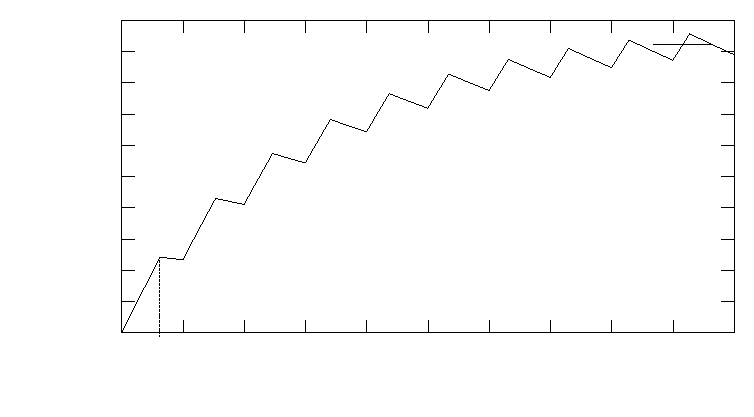
\includegraphics{./figure/simuCS}%
\end{picture}%
\begingroup
\setlength{\unitlength}{0.0200bp}%
\begin{picture}(18000,10800)(0,0)%
\put(2200,1650){\makebox(0,0)[r]{\strut{} 0}}%
\put(2200,2400){\makebox(0,0)[r]{\strut{} 0.5}}%
\put(2200,3150){\makebox(0,0)[r]{\strut{} 1}}%
\put(2200,3900){\makebox(0,0)[r]{\strut{} 1.5}}%
\put(2200,4650){\makebox(0,0)[r]{\strut{} 2}}%
\put(2200,5400){\makebox(0,0)[r]{\strut{} 2.5}}%
\put(2200,6150){\makebox(0,0)[r]{\strut{} 3}}%
\put(2200,6900){\makebox(0,0)[r]{\strut{} 3.5}}%
\put(2200,7650){\makebox(0,0)[r]{\strut{} 4}}%
\put(2200,8400){\makebox(0,0)[r]{\strut{} 4.5}}%
\put(2200,9150){\makebox(0,0)[r]{\strut{} 5}}%
\put(2475,1100){\makebox(0,0){\strut{} 0}}%
\put(3345,1200){\makebox(0,0){\strut{} $t_s$}}%
\put(3945,1100){\makebox(0,0){\strut{} 200}}%
\put(5415,1100){\makebox(0,0){\strut{} 400}}%
\put(6885,1100){\makebox(0,0){\strut{} 600}}%
\put(8355,1100){\makebox(0,0){\strut{} 800}}%
\put(9825,1100){\makebox(0,0){\strut{} 1000}}%
\put(11295,1100){\makebox(0,0){\strut{} 1200}}%
\put(12765,1100){\makebox(0,0){\strut{} 1400}}%
\put(14235,1100){\makebox(0,0){\strut{} 1600}}%
\put(15705,1100){\makebox(0,0){\strut{} 1800}}%
\put(17175,1100){\makebox(0,0){\strut{} 2000}}%
\put(550,5400){\rotatebox{0}{\makebox(0,0){\strut{}$I_L$}}}%
\put(9825,275){\makebox(0,0){\strut{}time ($10^{-7}s$)}}%
\put(9825,9975){\makebox(0,0){\strut{}switched circuit}}%
\end{picture}%
\endgroup
\endinput
  
  \label{fig:SIMU_CS}
 \end{figure}

 In \cite{maffezzoni2006}, it has been chosen that the NR iterations failed when the state of the
 diode and of the switch change at $t=t_s$. Indeed, the linearization performed at each NR iteration leads to an oscillation between two incorrect
 states and never converge to the correct one. The NR iterations enter in a infinite loop without converge. \\
 Using our formulation, because of the implicit time integration of the complementarity unknowns, the solving of the non-smooth problem find the correct state.

 

\section{Results on the buck converter}
\label{section4}
\begin{figure}[h]
\centerline{
 \scalebox{1.0}{
    \input{./figure/buck.pstex_t}
 }
}
\caption{Buck converter}
\label{fig-Buck-converter}
\end{figure}
The components are modelled with either linear or piecewise linear or set-valued relations yielding a non-smooth dynamical system of the linear time invariant complementarity systems class. The features of these models are given thereafter :
\paragraph{Power MOSFETS PMOS/NMOS:} they are described as an assembly of a
piecewise linear current source $I_{DS} = f(V_{GS}, V_{DS})$ and the intrinsic diode
(DPMOS and DNMOS) with an ideal characteristic.
The capacitances were not taken into account. The diodes threshold is
1 V. The MOSFETs transconductance KP was set to $10 AV^{-2}$ and
their threshold voltage to respectively -2 V for the PMOS and 2 V for
the NMOS. One can notice that the sum of their absolute values largely
exceeds the supply voltage $V_{I} = 3 V$ , thus providing non-overlapping
conduction times.
\paragraph{Compensator amplifier:} is modelled as a 10000 gain and an output low-pass
filter with a cutoff frequency of 30 MHz.
\paragraph{Comparator:} is modelled as a piecewise linear function whose value is 0 if
$x < -0.15V$ and 3 if $x > 0.15V$ .
\paragraph{Ramp voltage:} the frequency is 600 kHz and the bounds are 0 and 0.75 VI = 2.25 V .
The rise time is 1.655 us and the fall time is 10 ns.
\paragraph{Other components:} $V_I = 3 V , L = 10 \micro H, C = 22 \micro F,R_{load} = 10,$ compensator
: $R_{11} = 15.58 \kilo \ohm , R_{12} = 227.8 \kilo \ohm ,R_{21} = 5.613 \mega \ohm, C_{11} = 20 \pico F, C_{21} =
1.9 \pico F$
The reference voltage Vref rises from 0 to 1.8 V in 0.1 ms at the beginning
of the simulation.
The output voltage Voutput is regulated to track the reference voltage Vref when
VI or Vref or the load current vary. The error voltage Verror is a filtered value
of the difference between Voutput and Vref . This voltage signal is converted
into a time length thanks to a comparison with the periodic ramp signal. The
comparator drives the PMOS transistor which in turn provides more or less
charge to the output depending on the error level. The operation of a buck
converter involves both a relatively slow dynamics when the switching elements
(MOS and diodes) are keeping their conducting state, and a fast dynamics when
the states change. The order of magnitude are $ 50 \pico s$ for some switching details,
1 us for a slow variation period and $100 \micro s$ at least for a settling period of the
whole circuit requiring a simulation.
\subsection{The dynamical equations}
\label{section41}
The non-smooth DAE has been generated using the automatic circuit equation formulation describe in
\ref{fig:acef_algo}. It leads to a dynamical system of 25 unknowns connected to a inclusion rule. The dimension of the inclusion
rule depends on the MOS model. It could be 12 with a approximation of 2 segments, or 24 using the
model \ref{eq:68}.  

\subsection{Numerical results with {\sc siconos},  and comparisons}
\label{section42}
\subsubsection{Simulation with SICONOS}
 The start-up of the converter was simulated thanks to the SICONOS platform
developed at INRIA. As initial conditions, all state variables are zeroed.
The detailed analysis of the switching events requires to use a time step as
small as $50 \pico s$. The simulations are carried with a fixed time step, 4000000 steps
are then computed for the $200 \micro s$ long settling of the output voltage.
The overall result is shown on the figure \ref{fig:figSimuBuck} .\\
\textbf{The CPU time required to achieve the simulation is 60 seconds on a
Pentium 4 processor clocked at 3 GHz.} It includes 19 seconds in the MLCP solvers, 40 seconds in
matrix product. The time to export the resulting data is not include.
\begin{figure}[h]
  \centering
   \scalebox{0.6}{
  \input{./figure/BuckSimu.pstex_t}
  }
  \caption{Buck simulation}
  \label{fig:figSimuBuck}
\end{figure}

\begin{enumerate}
  \item[--] The figure \ref{fig:figSimuBuck} (a) is the output potential, following the ramp $V_{ref}$.
    \item[--] The figure \ref{fig:figSimuBuck} (b) is the current throw the inductor. Until $0.0001s$, $I_L$
    is loading the capacitor C. After $0.0001s$, $I_L$ has to keep constant the capacitor charge.
    \item[--] The figure \ref{fig:figSimuBuck} (c) zooms on the MOSP drain potential with standard
    parameters.
    \item[--] The figure  \ref{fig:figSimuBuck} (d) zooms on the MOSP drain potential with, $L=4\micro H,
    C=10\micro F,
    R_{11}=10\kilo \ohm, R_{21}=8\kilo \ohm ,C_{11}=10\pico F$, exhibiting a
    sliding mode 
  \end{enumerate}

The simulation has been tested with many parameters values. The robustness of the non-smooth modelling and solving algorithms enables to perform with the same
CPU time the simulation of such cases. 

\subsubsection{Simulation with SPICE }
\paragraph{Simulation conditions: convergence issues related to the MOS model}
The simulation of this circuit was done with several versions of SPICE (the open source NGSPICE from Berkeley, SMASH from Dolphin and
ELDO from Mentor Graphics) and two kinds of MOS models :
\begin{description}
\item[the MOS level 3 model :] this model was preferred to the MOS level 1 since it allowed the convergence
of the SMASH simulator with the requirement to add a small capacitor between ground and node 2 (connection between
the MOS transistors). This model takes more physical effects into account than the piecewise linear model used in SICONOS simulations,
in particular the voltage-dependent capacitances. It is an important issue since these varying capacitances
cause some convergence problems when node 2 switches between $V_I$ and ground.
Adding a small capacitor of a few picoFarad between this node and ground helps to solve the problem
but may yield artifacts (spikes) on the current of the~$V_I$~alim and the MOS transistors.
\item[a simplified model (Sah model)] with fixed capacitances and a quadratic static characteristic :
\[
I_{DS} = \textrm{max}(0,V_{GS}-Vt_N)^2 - \textrm{max}(0,V_{GD}-Vt_N)^2 \qquad \textrm{for an NMOS}
\]
This model is very close to the piecewise linear model used in SICONOS simulations. The implementation in netlists was done thanks to 
voltage-dependent current sources that are very likely not compiled by the various SPICE simulators tested.
Thus the CPU time measured is increased with respect to a compiled version of the same model.
An estimation of the CPU time with a compiled simplified model is given by multiplying the MOS level 3 CPU time
by the ratio of the Newton-Raphson iterations required respectively during the simulations with each model.
An additional correction should be done to reflect that the computation of the jacobian matrix entries
linked to a compiled simplified model would require less time than with a MOS level 3 model. Even if the SPICE simulation
includes other operations, jacobian matrix loading time is indeed known to be generally predominant.
\end{description}


\begin{itemize}
\item Power MOSFETS intrinsic diodes are modelled by the classical Shockley equation with an emission
coefficient $N~=~1$ :
\[ I = I_S.({e^{\frac{q.V}{N.k.T}} - 1}) \qquad \textrm{when} \quad V > -5.N.\frac{k.T}{q} \]
\[ I = -I_S \qquad  \textrm{when} \quad V < -5.N.\frac{k.T}{q} \]
with
\[
\begin{array}{ll}
V\,,\,I & \textrm{voltage across the diode and current through the diode}\\
I_S & \textrm{saturation current, default value $10^{-14}$~A}\\
q & \textrm{electron charge $1.6\,10^{-19}$~C}\\
k & \textrm{Boltzmann constant $1.38\,10^{-23}\,J.K^{-1}$}\\
T & \textrm{temperature in K}\\
N & \textrm{emission coefficient}
\end{array}
\]
\item The comparator is modelled as a non linear voltage controlled voltage source defined as $V_{out}~=~1.5~\cdot~(tanh(10~\cdot~V_{in}) + 1)$.
Thus the 3~segment characteristic used as the non smooth model is regularized to help convergence of SPICE
(see a comparison of the PWL comparator as used in SICONOS simulations with the SPICE one in figure \ref{fig-comparator-models}).
\end{itemize}

\begin{figure}[hbtp]
\begin{center}
\includegraphics[scale=1.0,angle=0]{./figure/comparators.eps}
\end{center}
\caption{Comparison of PWL and SPICE (tanh based) comparator models}
\label{fig-comparator-models}
\end{figure}

\clearpage

The power supply $V_I$ is raised from 0 in $50~ns$ at the beginning to help the convergence.\footnote{This is
not required with the SICONOS algorithms that find a consistent initial solution from scratch.}
The SPICE tolerance values used are $1~nA$ for currents, $1~\mu V$ for voltages and $0.00075$ for relative differences.
The maximum number of Newton-Raphson iterations is set to 100 (the default values are 10 for NGSPICE, 20 for SMASH and
13 for ELDO).

Usually, SPICE simulators integrate time with a time step adjusted according to different strategies based on an estimation
of the local truncation error (LTE) or the number of Newton-Raphson iterations required by previous steps.
Since SICONOS simulations were carried with a fixed time step of~50~ps, simulators were forced to use this value as a maximum.
Even when SPICE simulators use fixed time step, they may compute LTE to assess a solution found by the Newton-Raphson
algorithm. This computation of LTE was disabled because it could impair the performance of SPICE with respect to SICONOS.
\footnote{For NGSPICE, it implied a slight modification of the source code since no standard option is provided to do it.}

\subsubsection{Simulation comparisons}
The following tables displays the results with the standard and the sliding mode values of compensator components. An estimation of the CPU time with a compiled simplified model is added.
\\
\\
\begin{tabular}{|l|c|r|r|r|r|}
\hline
\multicolumn{6}{|c|}{\textbf{standard compensator values}}\\
\hline
simulator & model & time steps & NR iterations & CPU time (s) & CPU time estimation (s)\\
\hline
NGSPICE & simple  & 4000000 & 8024814 & 632 & 357\\
NGSPICE & level 3 & 4000000 & 8304237 & 370 & \\
\hline
SMASH   & simple  & 4000404 & 8073070 & 230 & 172\\
SMASH   & level 3 & 4000323 & 8059868 & 172 & \\
\hline
ELDO    & simple  & 4000000 & 4547579 & 388 & 355\\
ELDO    & level 3 & 4000000 & 4554452 & 356 & \\
\hline
\end{tabular}\\
\begin{tabular}{|l|c|r|r|r|r|}
\hline
\multicolumn{6}{|c|}{\textbf{sliding mode compensator values}}\\
\hline
simulator & model & time steps & NR iterations & CPU time (s) & CPU time estimation (s)\\
\hline
NGSPICE & simple  & 4000000 & 8070324 & 638 & 358\\
NGSPICE & level 3 & 4000000 & 8669053 & 385 & \\
\hline
SMASH   & simple  & 4000252 & 8239697 & 234 & 176\\
SMASH   & level 3 & 4000131 & 8220181 & 176 & \\
\hline
ELDO    & simple  & 4000000 & 5861226 & 438 & 365\\
ELDO    & level 3 & 4000000 & 5888994 & 367 & \\
\hline
\end{tabular}
\\
\\
These results shall be compared to the 60~s~CPU time achieved with the non-smooth dynamics.
Depending on the model and the SPICE simulator, the (estimated) CPU time is from~2.8~to~6.1
larger than with SICONOS.\\

Moreover, it was necessary to add a parasitic capacitor on the connection between the PMOS and NMOS
transistors to allow the convergence of the SMASH simulator with both models of MOS
and of the NGSPICE simulator with the MOS level 3 model.


\section{Conclusions}
\label{section5}


In this paper we have presented numerical simulations of switched circuits obtained with a suitable time-stepping implicit method, named Moreau's time-stepping algorithm. This method is based on the non-smooth dynamical systems modelling approach, and relies heavily on complementarity problems (equivalently, inclusions into normal cones) solvers. The advantages of such a method are that it allows one to:

\begin{itemize}

\item avoid computing the dynamics changes due to topology variations, since the circuits are treated as a global system with a fixed state dimension; modes transitions are taken care of by the complementarity problem solvers, which usually are polynomial in time;

\item simulate circuits with very large number of events without slowing down too much the simulation;

\item avoid regularization and consequently stiff systems of ODEs;

\item accurately calculate the initial steady-state of the system;

\item accurately simulate sliding mode trajectories without spurious oscillations around the switching surface;

\item compute state jumps (initial jumps due to inconsistent states, or in the course of the integration). 

\end{itemize}


The major drawback of the used method is its low order, so that its accuracy may be less good on smooth portions of the trajectoires. In this paper it is first shown that Moreau's time stepping scheme allows one to integrate an academic example on which Newton-Raphson based methods fail. Then the buck converter system is simulated. Comparisons with other analog simulators are presented. The simulations have been led with the {\sc siconos} software package of the INRIA, an open source platform dedicated to non-smooth dynamical systems. 


\bibliographystyle{plain}
\bibliography{CircuitSimulation}











\end{document}
%%% Local Variables: 
%%% mode: latex
%%% TeX-master: t
%%% End: 
